% Latex template: mahmoud.s.fahmy@students.kasralainy.edu.eg
% For more details: https://www.sharelatex.com/learn/Beamer

\documentclass[aspectratio=1610]{beamer}					% Document class

\setbeamertemplate{footline}[text line]{%
  \parbox{\linewidth}{\vspace*{-8pt}Statistical analysis for ensemble snapshots of transcriptional bursting \hfill\insertshortauthor\hfill\insertpagenumber}}
\setbeamertemplate{navigation symbols}{}

\usepackage[english]{babel}				% Set language
\usepackage[utf8x]{inputenc}			% Set encoding

\mode<presentation>						% Set options
{
  \usetheme{default}					% Set theme
  \usecolortheme{default} 				% Set colors
  \usefonttheme{default}  				% Set font theme
  \setbeamertemplate{caption}[numbered]	% Set caption to be numbered
}

% Uncomment this to have the outline at the beginning of each section highlighted.
%\AtBeginSection[]
%{
%  \begin{frame}{Outline}
%    \tableofcontents[currentsection]
%  \end{frame}
\usepackage{graphicx}					% For including figures
\usepackage{booktabs}					% For table rules
\usepackage{hyperref}	
\usepackage{tikz-network}				% For cross-referencing
\usepackage[absolute,overlay]{textpos}
\usepackage{bm}
\usepackage[font=small,labelfont=bf]{caption}				% For cross-referencing

\title{Statistical analysis for ensemble snapshots of transcriptional bursting}	% Presentation title
\author{Clayton W. Seitz}								% Presentation author
\date{\today}									% Today's date	

\begin{document}

% Title page
% This page includes the informations defined earlier including title, author/s, affiliation/s and the date
\begin{frame}
  \titlepage
\end{frame}


% The following is the most frequently used slide types in beamer
% The slide structure is as follows:
%
%\begin{frame}{<slide-title>}
%	<content>
%\end{frame}



\begin{frame}{Gene expression is stochastic and non-constitutive}


\begin{textblock*}{7cm}(1cm,1cm)
\begin{figure}
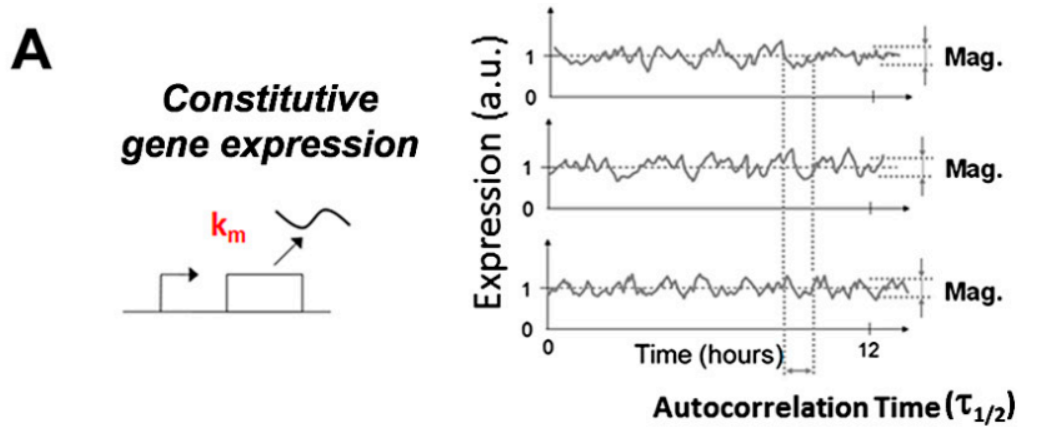
\includegraphics[width=7cm]{burst-1.png}
\end{figure}
\end{textblock*}

\begin{textblock*}{7cm}(8cm,1cm)
\begin{figure}
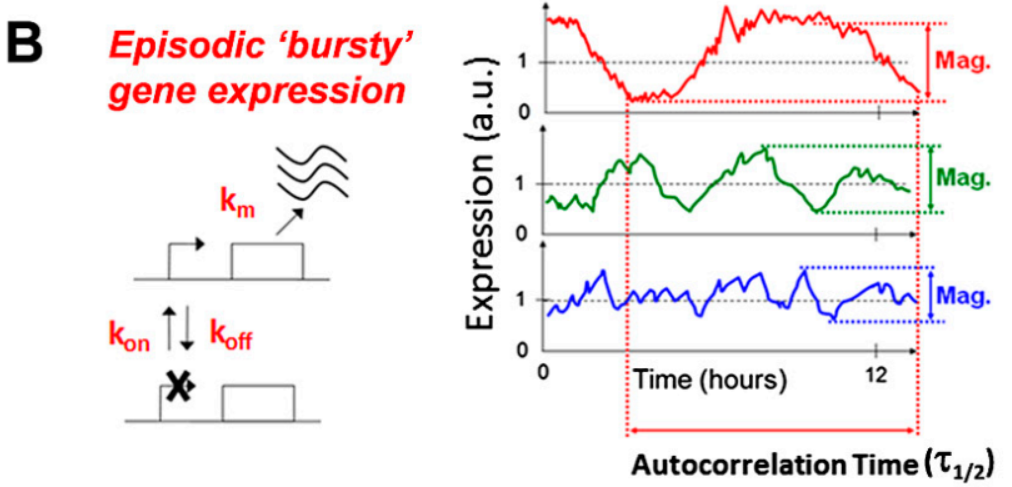
\includegraphics[width=6cm]{burst-2.png}
\end{figure}
\end{textblock*}


\begin{textblock*}{6cm}(1cm,5cm)
\hspace{0.5in}\textbf{Single-state models}
\begin{itemize}
\item RNAs are 'born' at a fixed rate
\item RNA counts are Poisson
\end{itemize}
\end{textblock*}

\begin{textblock*}{6cm}(8cm,5cm)
\hspace{0.5in}\textbf{Multi-state models}
\begin{itemize}
\item Promoter can be in multiple states
\item RNA counts are not Poissonian
\end{itemize}

\end{textblock*}

\begin{textblock*}{15cm}(0.5cm,8cm)
Single-state models tend to \textcolor{red}{underestimate variance in RNA counts}
\end{textblock*}


\end{frame}

\begin{frame}

We would like to investigate transcriptional bursting using fluorescence in-situ hybridization (FISH)\\
\vspace{0.2in}

\begin{itemize}
\item Our image acquisition and detection strategy is standardized (5 by 5 regions, max-intensity z-projections, LoG blob detection and 2D Gaussian fitting)
\item Need to identify a set of target genes, which we have good reason to believe are under the control of our treatment condition and not expressed constitutively
\item Aiming for ~3000 cells (for each treatment condition?)
\item Need to define a cell-line (HeLa?) and treatment condition pairing
\item \textcolor{red}{Need to define a set of analysis methods compatible with ensemble snapshot data}
\end{itemize}

\end{frame}

\begin{frame}{Testing dataset:  STL1/CTT1 induction with NaCl in yeast}
\begin{textblock*}{12cm}(2cm,1.25cm)
\begin{figure}
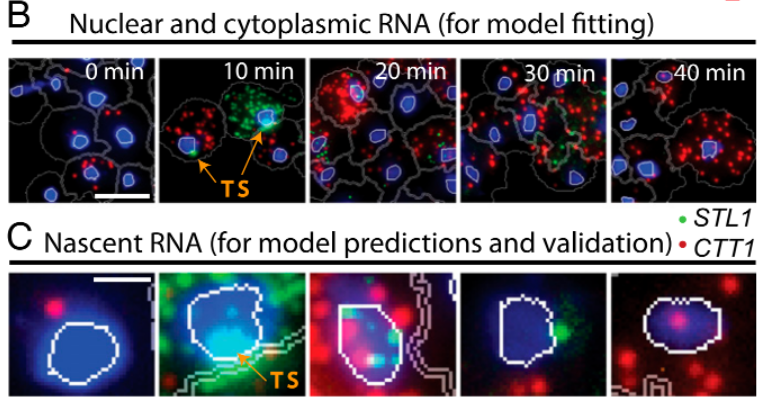
\includegraphics[width=12cm]{salt.png}
\caption{Munsky et al., PNAS 2018}
\end{figure}
\end{textblock*}
\end{frame}


\begin{frame}{Testing dataset: STL1/CTT1 induction with NaCl in yeast}

Useful as a guide when designing our own experiments:
\vspace{0.2in}

\begin{itemize}
\item 0.2M NaCl
\begin{itemize}
\item 2 biological replicates
\begin{itemize}
\item 15 time points per replicate
\end{itemize}
\end{itemize}
\item 0.4M NaCl
\begin{itemize}
\item 3 biological replicates
\begin{itemize}
\item 15 time points per replicate
\end{itemize}
\end{itemize}
\end{itemize}

\end{frame}

\begin{frame}{STL1 mRNA counts per cell at 0.4M NaCl}

\begin{textblock*}{5cm}(3.4cm,0.75cm)
\begin{figure}
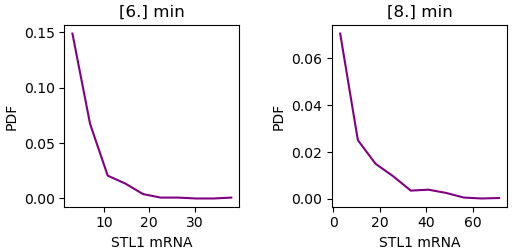
\includegraphics[width=9cm]{count-hist-2.png}
\end{figure}
\end{textblock*}

\begin{textblock*}{5cm}(3.4cm,4.5cm)
\begin{figure}
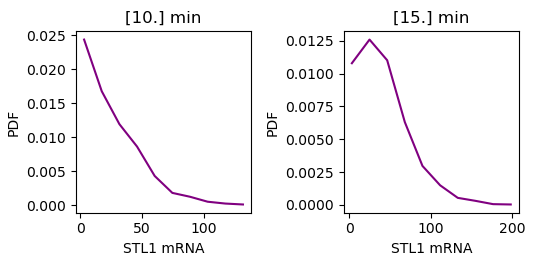
\includegraphics[width=9cm]{count-hist-1.png}
\end{figure}
\end{textblock*}

\end{frame}

\begin{frame}{STL1 mRNA counts per cell at 0.4M NaCl}

\begin{textblock*}{5cm}(3.25cm,0.5cm)
\begin{figure}
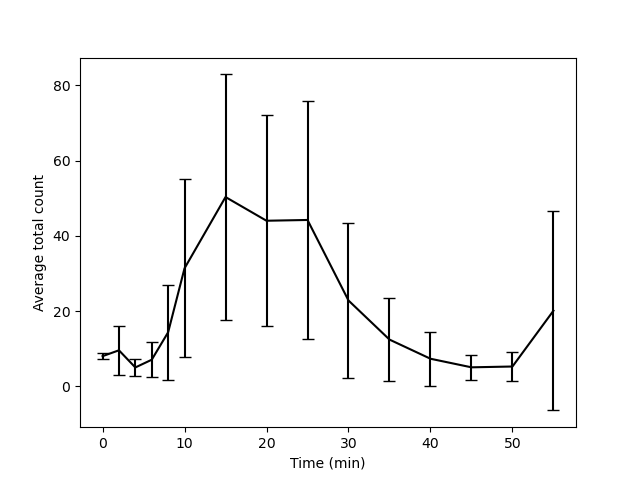
\includegraphics[width=10cm]{avg-count.png}
\end{figure}
\end{textblock*}

\vspace{7.25cm}
Error bars represent standard deviations from the mean. Cells marked ON for $>$ 3 STL1 mRNA

\end{frame}

\begin{frame}{Statistically defining the unit intensity}

\begin{textblock*}{5cm}(3.25cm,0.5cm)
\begin{figure}
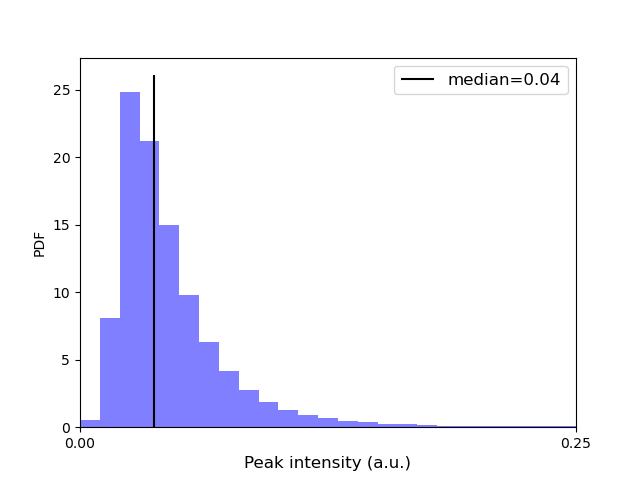
\includegraphics[width=10cm]{int-hist.png}
\end{figure}
\end{textblock*}

\vspace{7.25cm}
The median of the mRNA intensity distribution is used to determine the number of nascent RNA at the transcription site (TS)

\end{frame}

\begin{frame}{Nascent mRNA counts at the transcription site}

\begin{textblock*}{5cm}(0.75cm,1.5cm)
\begin{itemize}
\item Brightest spot in the nucleus defined as putative TS
\item TS marked ACTIVE if $I>2*\mathrm{med}$
\item Nascent mRNA count is $I/\mathrm{med}$
\end{itemize}

\end{textblock*}

\begin{textblock*}{5cm}(7cm,0.75cm)
\begin{figure}
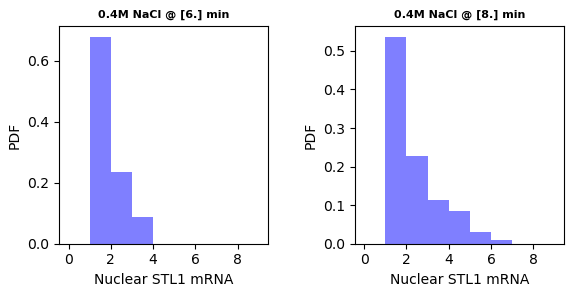
\includegraphics[width=8cm]{active-ts-dist-2.png}
\end{figure}
\end{textblock*}

\begin{textblock*}{5cm}(7cm,4.5cm)
\begin{figure}
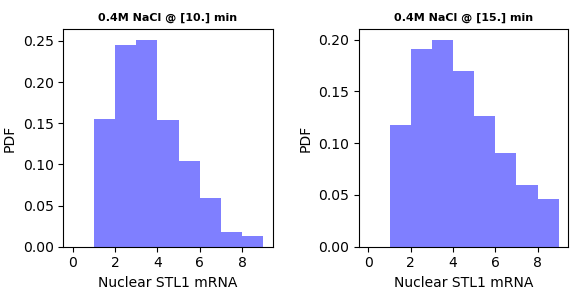
\includegraphics[width=8cm]{active-ts-dist-1.png}
\end{figure}
\end{textblock*}

\end{frame}


\begin{frame}{Comments}


\begin{itemize}
\item Average counts show a 'transcriptional burst', but variability is very high
\item Cells are not necessarily bursting synchronously
\item Ensemble averages may not accurately represent the underlying dynamics
\item How to correlate transcriptional bursting with spatial organization of transcripts?
\end{itemize}


\end{frame}

\end{document}